\documentclass[a4paper,12pt]{article}
\usepackage[left=1.5cm,right=1.5cm,
    top=1cm,bottom=1.5cm,bindingoffset=0cm]{geometry}

\usepackage[T1,T2A]{fontenc}
\usepackage[utf8]{inputenc}
\usepackage[english,russian,ukrainian]{babel}
\usepackage{tabularx}
\usepackage{amssymb}
\usepackage{color}
\usepackage{amsmath}
\usepackage{mathrsfs}
\usepackage{listings}
\lstset{language=Python, extendedchars=\true}
\usepackage{graphicx}
\graphicspath{ {./images/} }
%\usepackage{draftwatermark} не будет лезть на картинки
\usepackage[printwatermark]{xwatermark}%будет лезть на картинки
\usepackage{lipsum}
\usepackage{xcolor}
\usepackage{tikz}
%\newsavebox\mybox
%\savebox\mybox{\tikz[color=red,opacity=0.1]\node{AnMn.test};}
%\newwatermark*[allpages,angle=45,scale=11,xpos=-40, ypos=35]{\usebox\mybox}
\definecolor{lgreen}{rgb}{0.5,1,1}
\definecolor{n}{rgb}{1,0.5,0.5}
\definecolor{n1}{rgb}{1,1,0.5}
\definecolor{n3}{rgb}{1,0.7,0.9}
\usepackage{subcaption,floatrow,graphicx,calc}
\floatsetup{floatrowsep=qquad}



\begin{document}
\pagecolor{white}
\pagestyle{plain}
\begin{center}
   \begin{center} 
   \large{\textbf{Міністерство освіти і науки України} \par 
   \textbf{Національний технічний університет України}}\par
	“Київський політехнічний інститут”\par
	 Факультет електроніки\par
    	Кафедра мікроелектроніки\par
    \end{center}
    \vspace{4cm}
    
   	{\bfseries ЛАБОРАТОРНА РОБОТА № 1\par}
        \vspace{1cm}
        \large
        {
    	з курсу\par
    	«Теорія сигналів» \par
      	"Основи програмування мовою Python" \par  
	}
	\end{center}

       \vspace{7cm}
       \begin{tabularx}{\textwidth}{Xr}
        \flushright
           \begin{large} 
        Студента 3 курсу\par
 	групи ДП-81\par
	Фіцая Руслана\par
	 \end{large}
	\end{tabularx}
   
   \vfill
   \begin{center}
    {Київ} --- 2020
    \end{center}
%-----------------------------------------------------------------------------------------------------    
 \newpage   

\begin{center}
\textbf{Пункт 3}\par
\end{center}
Ознайомитися:\\
- з задаванням масиву, елементи якого є арифметичною послідовністю;\\
- з роботою функцій генерації випадкових чисел із заданими густинами розподілу імовірності. Ознайомитися з функцією побудови гістограм, побудувати гістограми випадкових чисел з різними розподілами густини ймовірності;\\

\lstinputlisting[language=Python]{gistogramm.py}

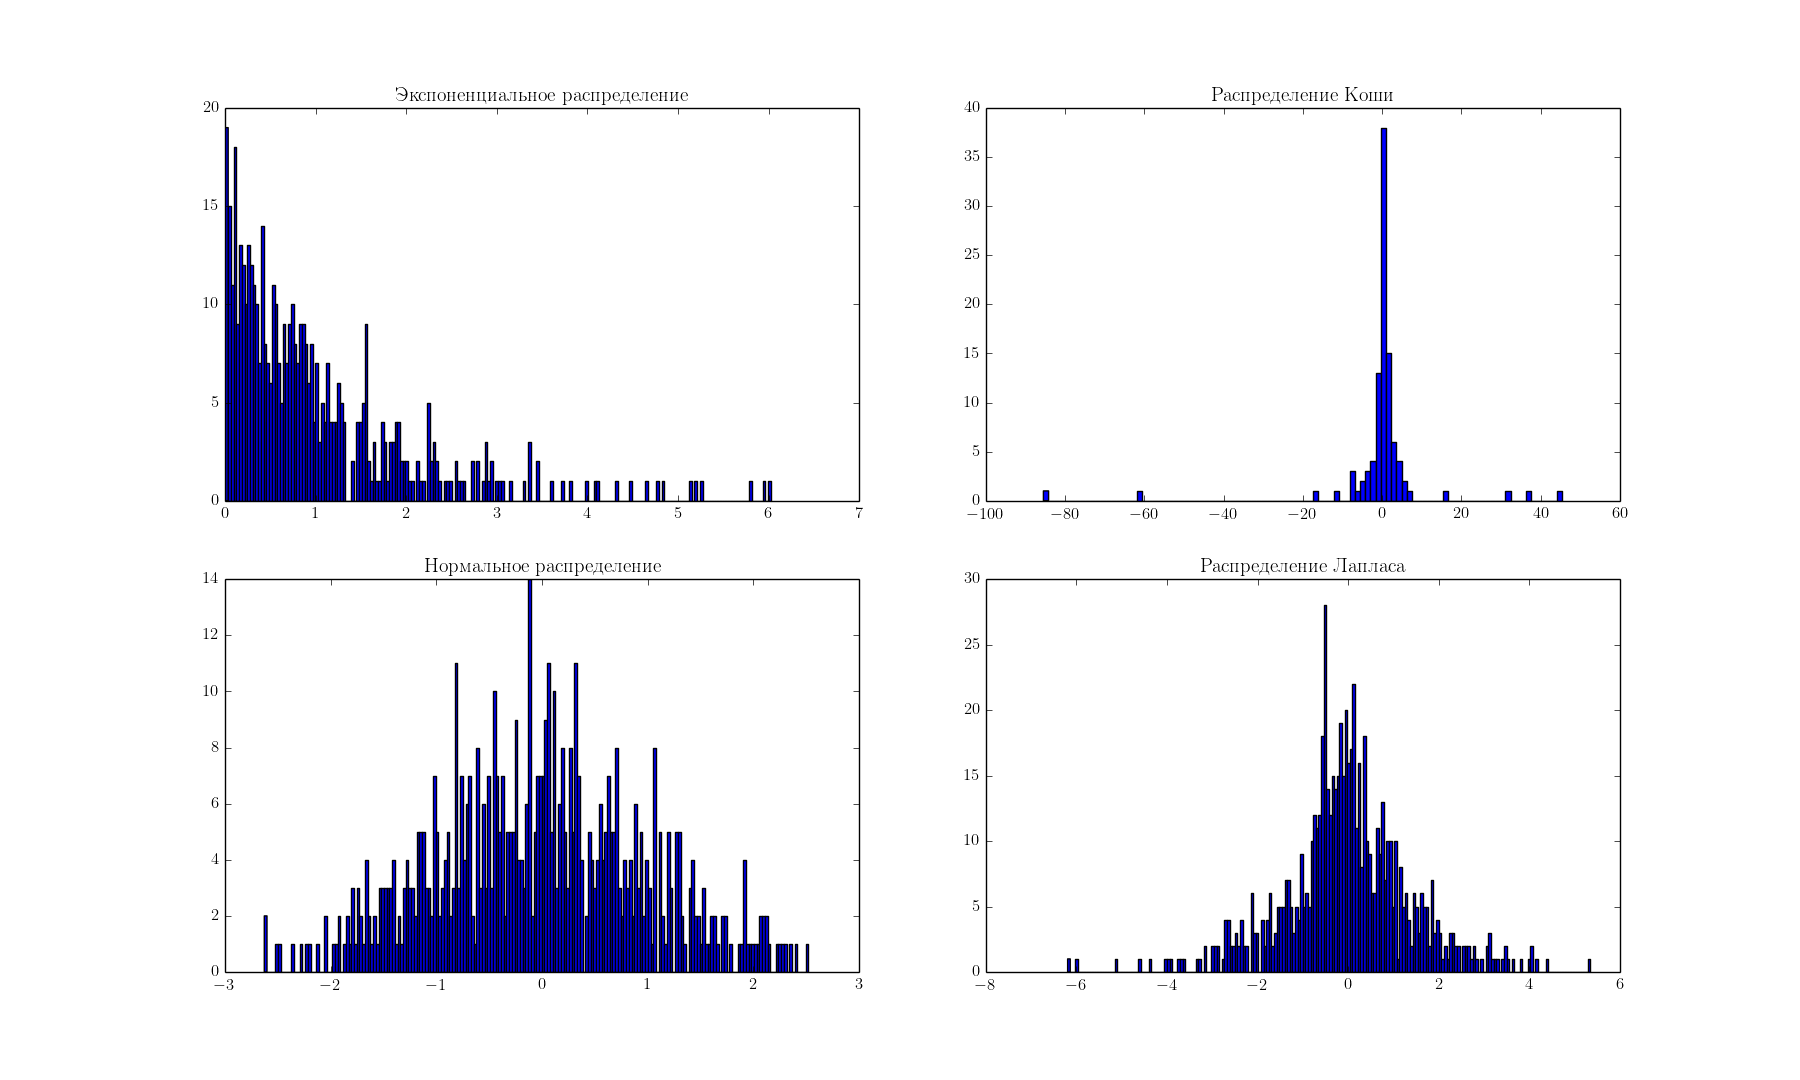
\includegraphics[trim=3cm 0 0 -0.5cm, height = 16 cm, width =  19 cm]{gistorramm.png}



\begin{center}
\textbf{Пункт 4}\par
\end{center}
Ознайомитися з написанням власних файлів-сценаріїв. У власному файлі-сценарії побудувати графік лінійної функції однієї змінної. Позначити вісі та заголовок графіку, нанести координатну сітку.\par
\lstinputlisting[language=Python]{4.py}
\begin{center}
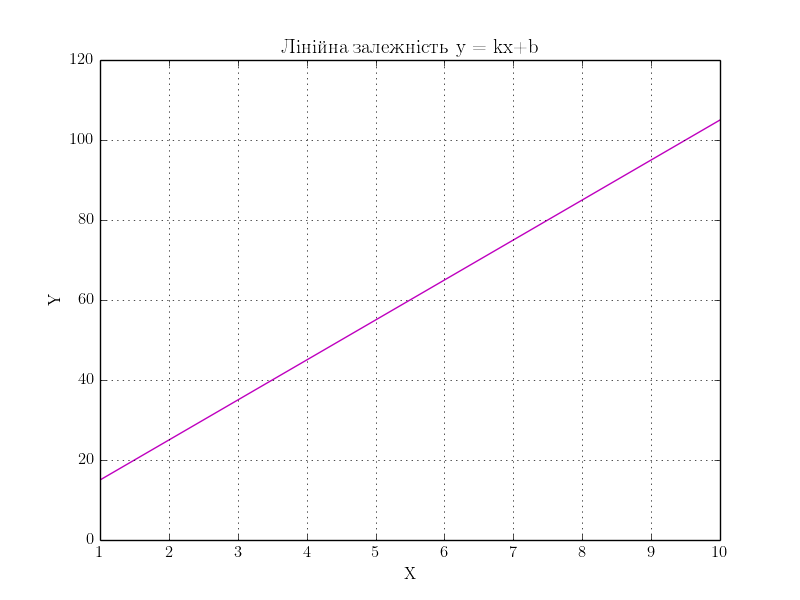
\includegraphics[height = 12 cm,width=14 cm]{4.png}
\end{center}
\vspace{1cm}\par



\begin{center}
\textbf{Пункт 5}\par
\end{center}
\textbf{5.1} Побудувати графіки синусоїд частот 1, 10, 50 Гц. Тривалість сигналів – 1 сек., частота дискретизації 256 Гц. Графіки будувати в одному вікні, але в різних осях. Амплітуди кожної синусоїди повинні бути випадковими числами.\par
\textbf{5.2} Виконати теж саме, але  задавати амплітуду кожної синусоїди з клавіатури.\par
\textbf{5.3} Підписати заголовок кожного графіку текстом, який буде містити значення частоти та амплітуди відповідної синусоїди.\par
\lstinputlisting[language=Python]{5.py}

\begin{center}
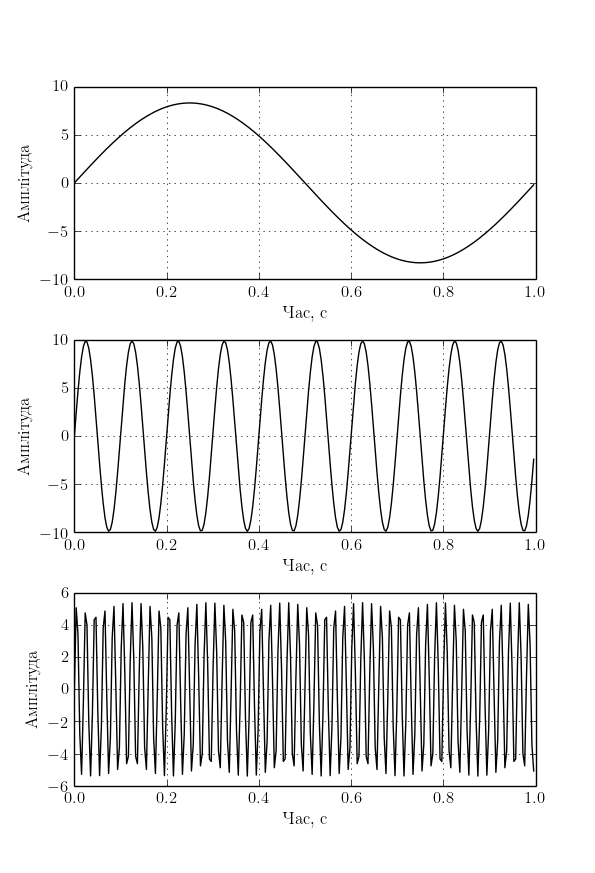
\includegraphics[height = 11.5 cm,width=13 cm]{5r.png}
\end{center}
%-----------------------------------------------------------------------------------------------------    
\begin{center}
\textbf{Пункт 6}\par
\end{center}

\textbf{6.1} Побудувати одиночний прямокутний імпульс. Задати проміжок значень часу 10 секунд, частота дискретизації 256 Гц. Побудувати графік одиничного прямокутного імпульсу шириною 300 мс, з центром в момент часу 4 с.\par

\lstinputlisting[language=Python]{6.1.py}

\begin{center}
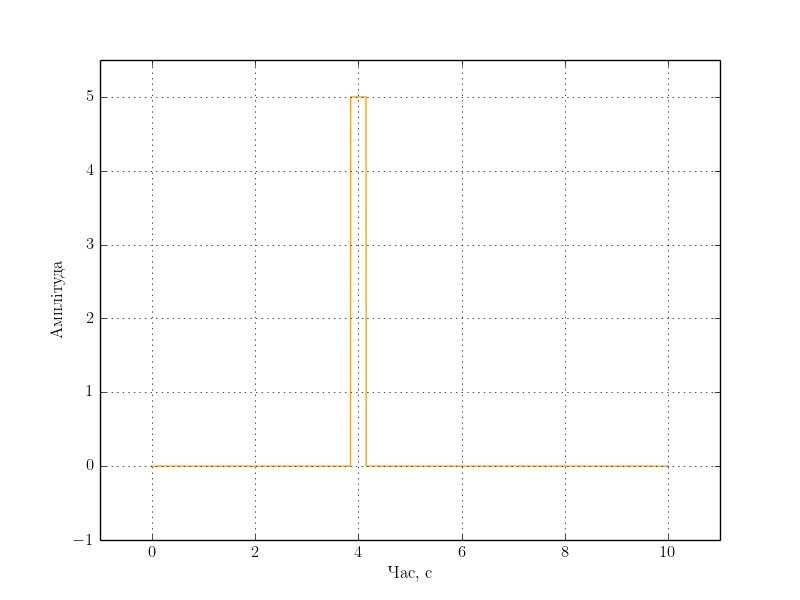
\includegraphics[height = 11.5 cm,width=15 cm]{6.1.png}
\end{center}

\textbf{6.2} Написати файл-сценарій для побудови графіку прямокутного імпульсу, тривалість та амплітуда якого буде задаватися з клавіатури. Розташування імпульсу задавати випадковим числом, але передбачити перевірку, чи не виходе імпульс за межі графіка.

\lstinputlisting[language=Python]{6.2prav.py}

\begin{center}
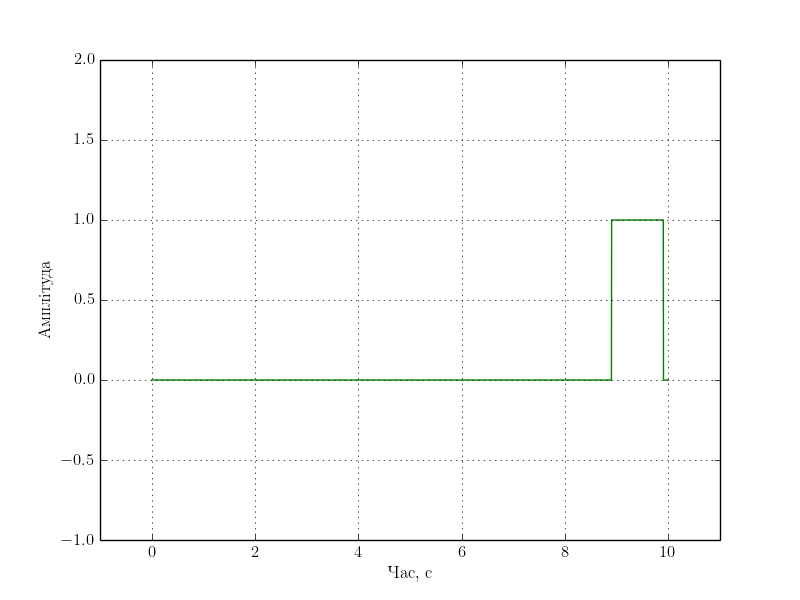
\includegraphics[height = 12 cm,width=15 cm]{6.2r.png}
\end{center}

\textbf{6.3} Побудувати послідовність прямокутних імпульсів для двох випадків: а) коли інтервали між імпульсами однакові, б) коли інтервали між імпульсами випадкові і задаються програмно.
\lstinputlisting[language=Python]{6.3.py}

\begin{center}
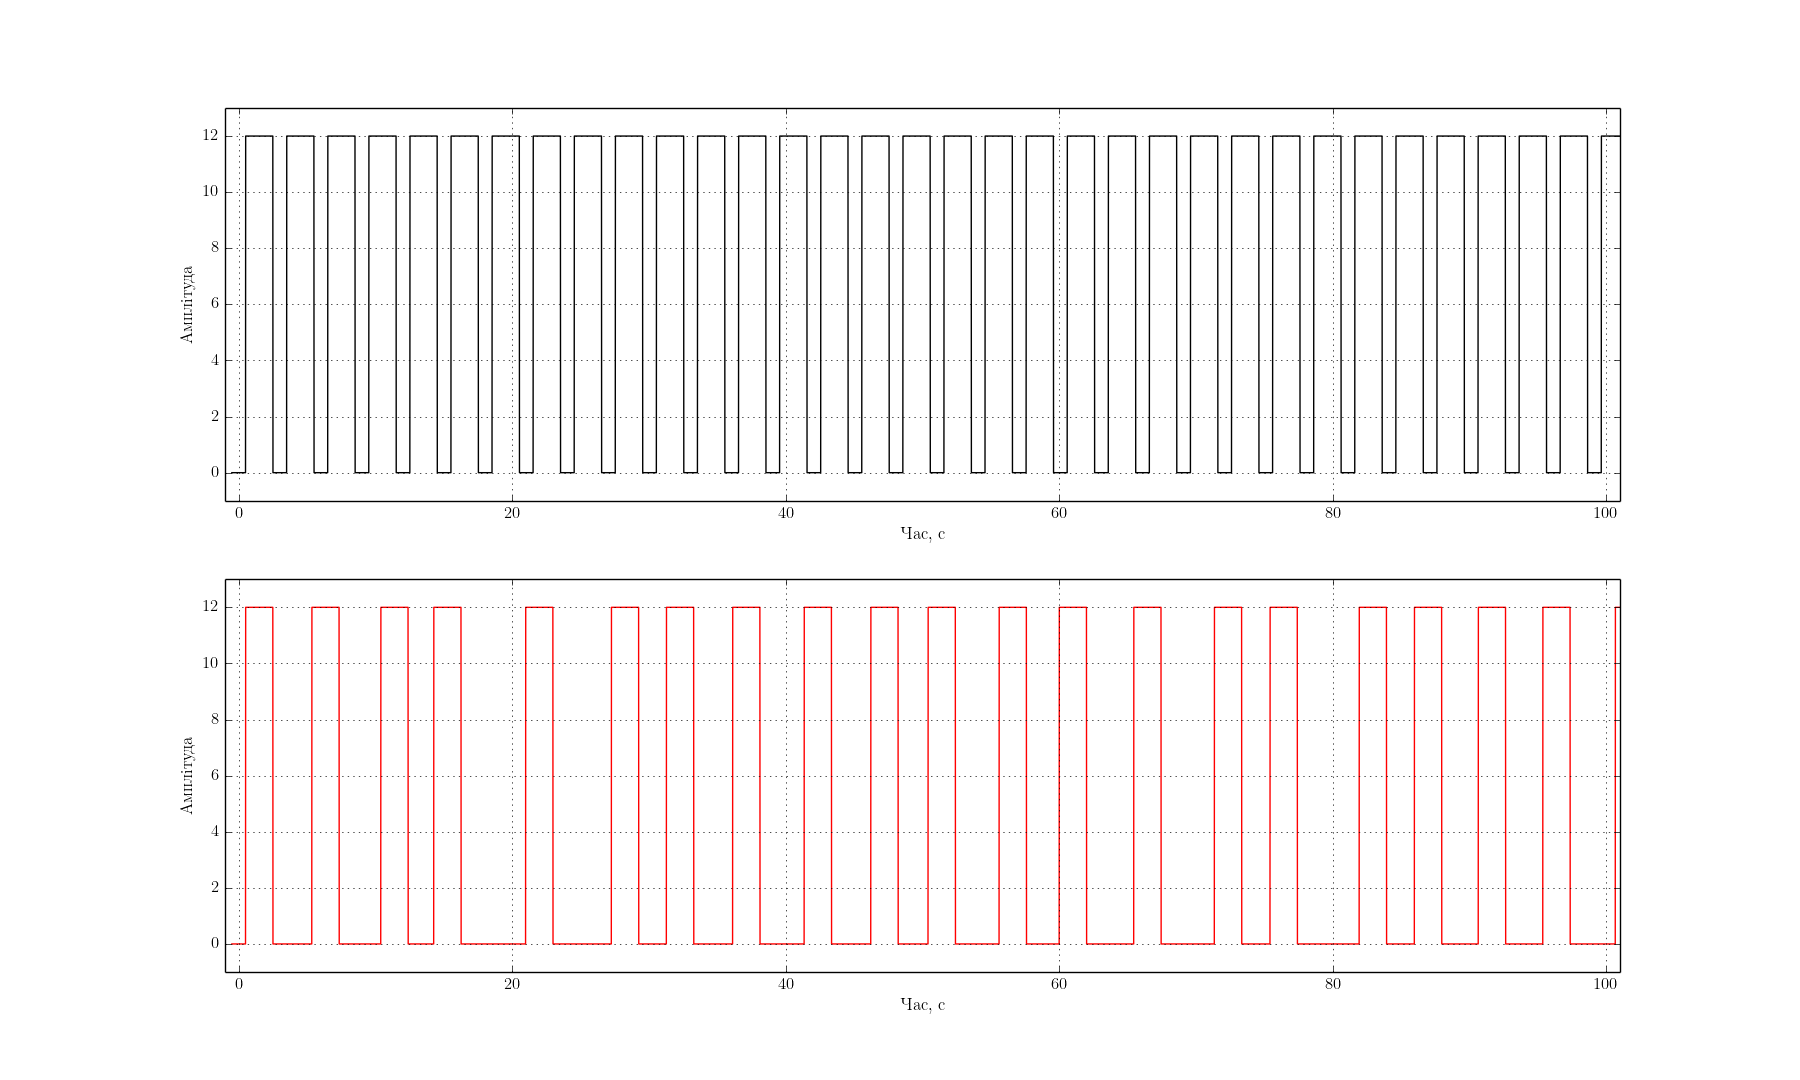
\includegraphics[height = 13 cm,width=16 cm]{6.3.png}
\end{center}
%________________________________________________



\begin{center}
\textbf{Пункт 7}\par
\end{center}
Зберегти дані розрахунку функції в файл. Прочитати їх із файлу в іншому сценарії, побудувати графік функції.\par

\lstinputlisting[language=Python]{7read_file.py}%\begin{center}
%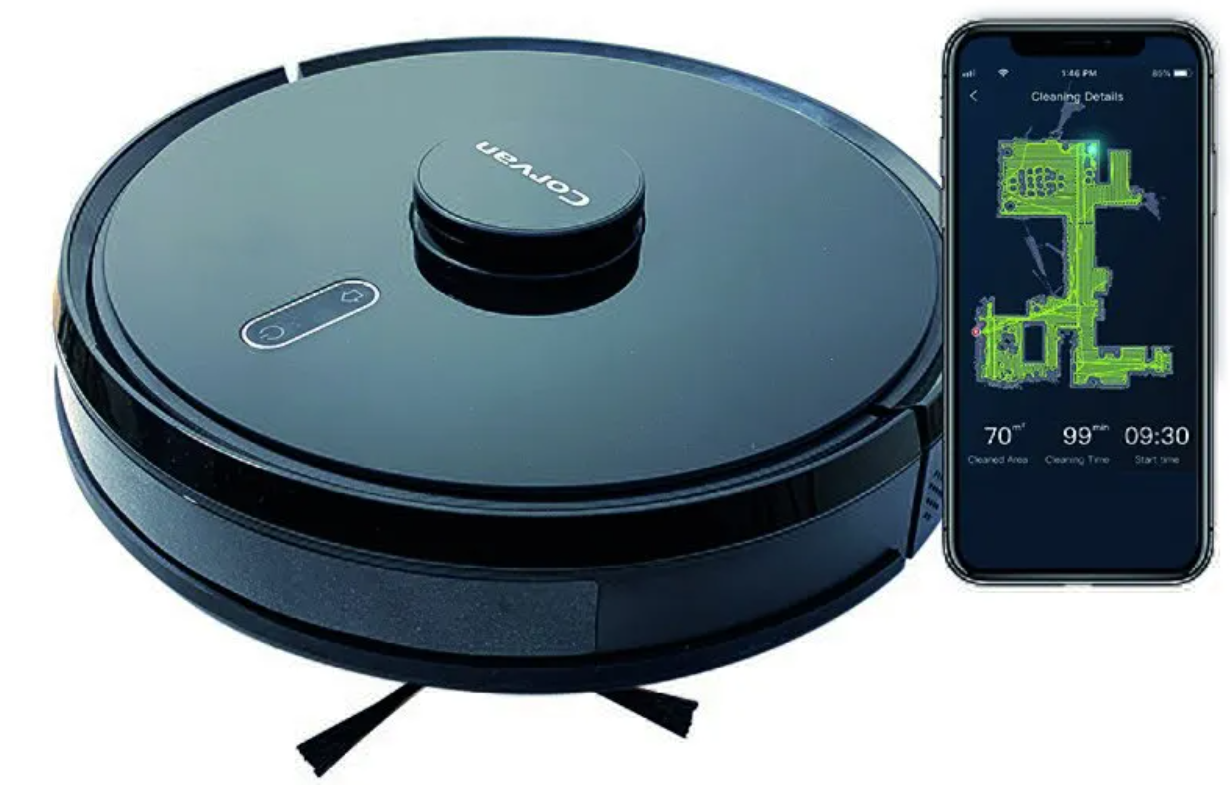
\includegraphics[height = 12 cm,width=15 cm]{7.png}

\begin{center}
{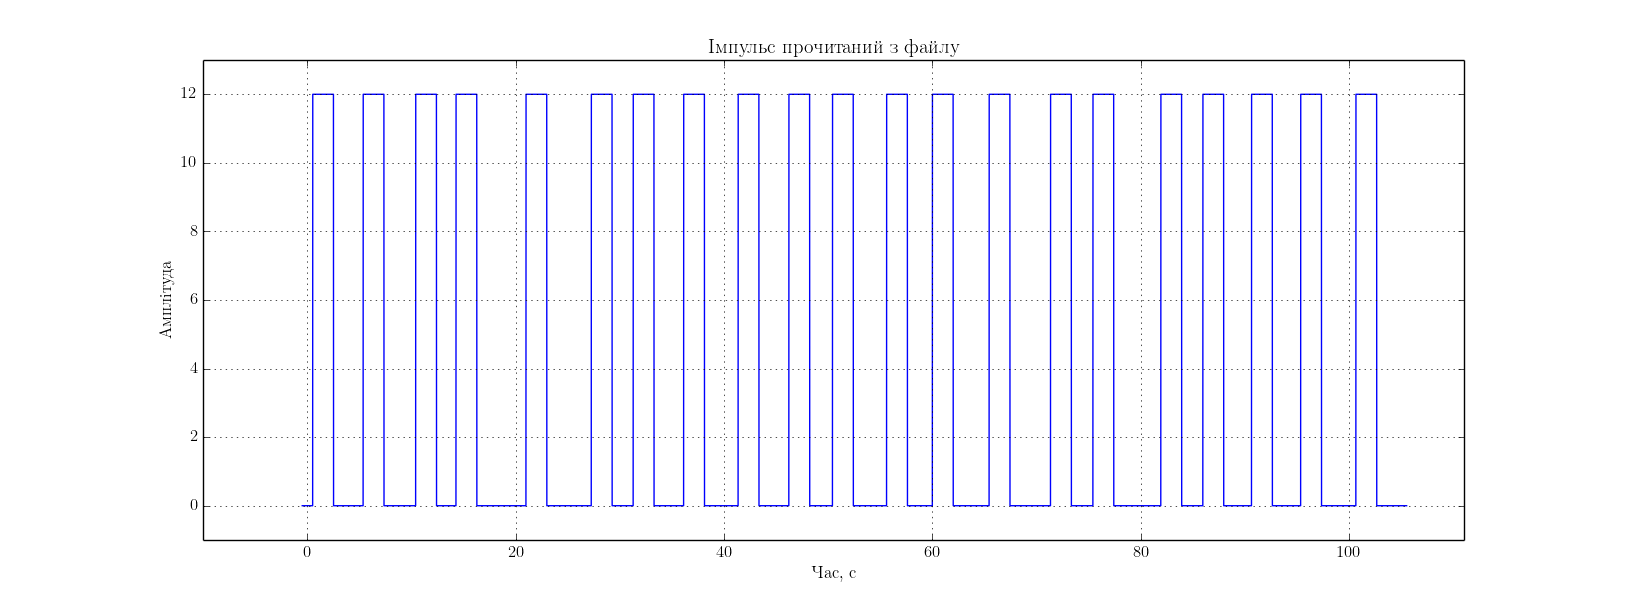
\includegraphics[height = 10 cm,width=13 cm]{7readen.png} }\\
\end{center}

\begin{center}
\textbf{Пункт 8}\par
\end{center}
 Побудувати власний файл-функцію для побудови графіка синусоїдального сигналу із заданою частотою, амплітудою та тривалістю для частоти дискретизації 256 Гц. В якості вихідного параметру функції вивести середнє значення синусоїди. \par

\lstinputlisting[language=Python]{8.py}
\begin{center}
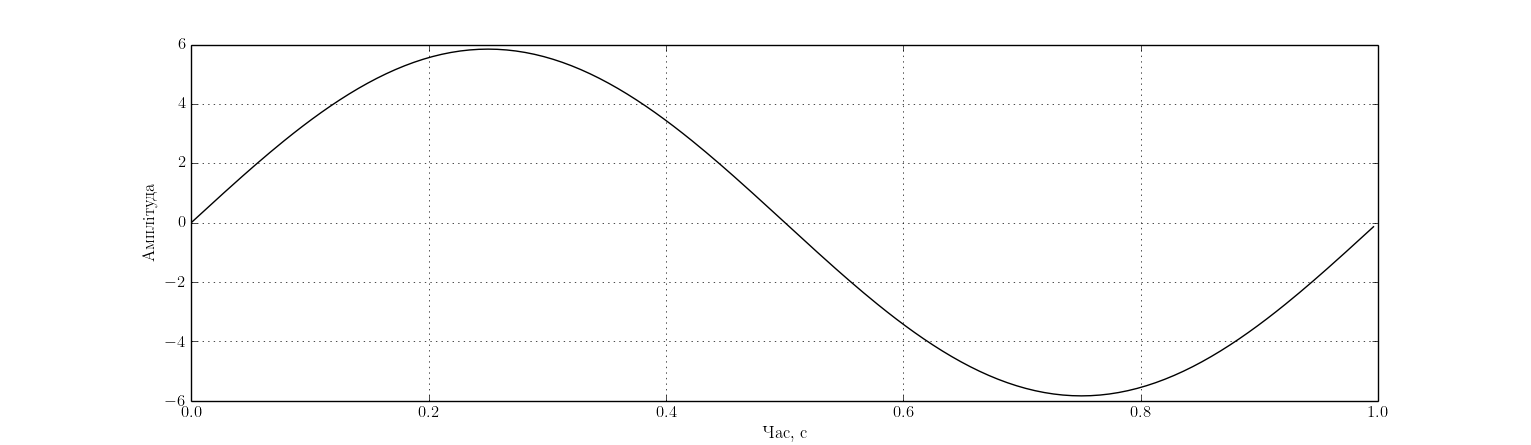
\includegraphics[height = 12 cm, width=18 cm]{8.png}\par
\vspace{1cm}
\end{center}
Cереднє значення синусоїди = 2.18





\end{document}